% Selbst erstelltes Mockup einer Kontakte-App mit erfundenen Namen und Nummern
% (ersetzt das frühere App-Symbol Contacts_1.png und den Screenshot Contacts_2.png).
% Namen passen zu den Listen auf den folgenden Folien (Anna, Ben, Clara).
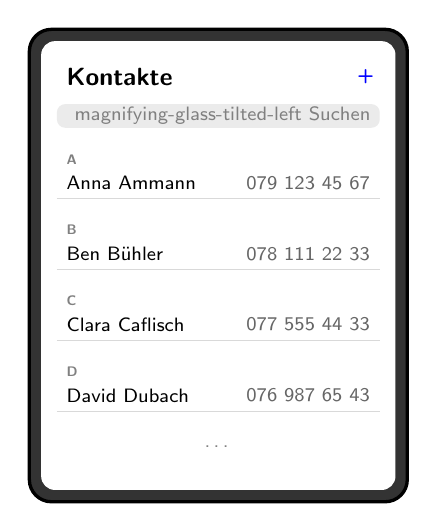
\begin{tikzpicture}[font=\sffamily\scriptsize]
	% Gerät und Bildschirm
	\draw[rounded corners=8pt, line width=1.2pt, fill=black!80] (0,0) rectangle (4.8,6);
	\fill[rounded corners=5pt, white] (.15,.15) rectangle (4.65,5.85);
	% Kopfzeile mit Titel und Suchfeld
	\node[anchor=west, font=\sffamily\bfseries\small] at (.35,5.4) {Kontakte};
	\node[anchor=east, text=blue] at (4.5,5.4) {\textbf{+}};
	\fill[rounded corners=3pt, black!8] (.35,4.75) rectangle (4.45,5.05);
	\node[anchor=west, text=black!50] at (.45,4.9) {\emoji{magnifying-glass-tilted-left} Suchen};
	% Einträge: Buchstabe als Zwischentitel, dann Name und Nummer
	\foreach \y/\buchstabe/\name/\nummer in {
			4.35/A/Anna Ammann/079 123 45 67,
			3.45/B/Ben Bühler/078 111 22 33,
			2.55/C/Clara Caflisch/077 555 44 33,
			1.65/D/David Dubach/076 987 65 43} {
			\node[anchor=west, text=black!50, font=\sffamily\tiny\bfseries] at (.35,\y) {\buchstabe};
			\node[anchor=west] at (.35,\y-.3) {\name};
			\node[anchor=east, text=black!60] at (4.45,\y-.3) {\nummer};
			\draw[black!15] (.35,\y-.5) -- (4.45,\y-.5);
		}
	\node[text=black!50] at (2.4,.7) {\ldots};
\end{tikzpicture}
